\documentclass[a4paper, 10pt]{article}
\usepackage[margin=1in]{geometry}
\usepackage[parfill]{parskip}          % skip a line instead of indenting new paragraphs
\usepackage{hyperref}
\hypersetup
{
  colorlinks=false,
  pdfborder={0,0,0},
}
 
\usepackage{fancyhdr}
\fancyhead[L]{\class \;- \assignment  \;- \duedate }
\fancyhead[R]{\author }
\renewcommand{\footrulewidth}{0.5pt} % Insert a line above the footer
\pagestyle{fancy}
\usepackage[hang,small,bf]{caption}
\usepackage{palatino}
\usepackage{amsmath}
\usepackage{amssymb}
\usepackage{enumerate}
\usepackage{graphicx}
 
% convenience commands
\renewcommand{\author}{Daniel Standage}
\newcommand{\class}{GDCB 511}
\newcommand{\instructor}{Yin/Yang}
\newcommand{\assignment}{Problem Set 6}
\newcommand{\duedate}{Apr 25, 2012}
 
\newcounter{prob_num}
\setcounter{prob_num}{1}
% usage: \problem
\newcommand{\problem}{\vspace{20pt}\arabic{prob_num}.\stepcounter{prob_num}\par}
% usage: \head{name}{class}{assignment}
\newcommand{\head}{\begin{center}\begin{tabular*}{\linewidth}{l@{\extracolsep{\fill}}r} & \class \;- \assignment \\ & \duedate \end{tabular*}\end{center} \hfill }
% usage: \eqn{equation}{label}
\newcommand{\eqn}[2]{\begin{equation}#1\label{#2}\end{equation}}
 
\begin{document}

%%%%%%%%%%%%%%%%%%%%%%%%%%%%%%%%%%%%%%%%%%%%%%%%%%
\problem
First, sequencing the protein and searching sequence databases for homologous proteins identified several proteins from both eukaryotes and prokaryotes that are involved in lesion-bypass DNA synthesis, including two genes from \textit{Saccharomyces cerevisiae} involved in error-free lesion-bypass activity. Additionally, an \textit{in vitro} damage bypass replication assay showed that XP-V cells could not undergo trans-lesion replication, but the addition of HeLa DNA Pol $\eta$ restored this activity.

%%%%%%%%%%%%%%%%%%%%%%%%%%%%%%%%%%%%%%%%%%%%%%%%%%
\problem
\begin{center}
  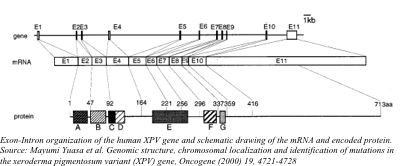
\includegraphics[width=250px]{xpv.png}
\end{center}

The 4 bands in the northern blot correspond to 4 different alternatively spliced isoforms of the gene.

%%%%%%%%%%%%%%%%%%%%%%%%%%%%%%%%%%%%%%%%%%%%%%%%%%
\problem
The inclusion of DNA Pol $\alpha$ enabled comparison of this polymerase's activity against that of DNA Pol $\eta$. On a 30 bp oligonucleotide containing a T-T dimer, the recombinant protein successfully bypassed the dimer, whereas the DNA Pol $\alpha$ stopped short and only synthesized 16-mers.

%%%%%%%%%%%%%%%%%%%%%%%%%%%%%%%%%%%%%%%%%%%%%%%%%%
\problem
XP-V carry a mutant form of the XPV gene, which codes for DNA Pol $\eta$. The mutant polymerase cannot bypass DNA damage caused by UV radiation, affecting its ability to replicate and therefore causing a lower sensitivity to UV radiation.

\end{document}
